\begin{exercise}
\begin{figure}[H]
\centering
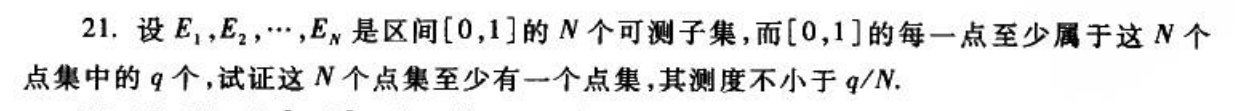
\includegraphics[width=\textwidth]{hw10-2025051210.png}
% \caption{}
\label{}
\end{figure}
\end{exercise}
\begin{proof}
Assume that $mE_i<q/N,\forall i\in \{ 1,\dots,N \}$. Since every point in $[0,1]$ belongs to at least $q$ of $E_1,\dots,E_{N}$, we have
\[
\sum_{i=1}^{N} \chi_{E_i}(x)\geq q\qquad \forall x\in[0,1]
\]
Then
\[
\int_{[0,1]}^{} \sum_{i=1}^{N} \chi_{E_i}(x) \, \mathrm{d}x \geq \int_{[0,1]}^{} q \, \mathrm{d}x =q
\]
\[
\sum_{i=1}^{N} \int_{[0,1]}^{} \chi_{E_i}(x) \, \mathrm{d}x =\sum_{i=1}^{N} m(E_i)<\sum_{i=1}^{N} \frac{q}{N}=q
\]
By the linearity of integral,
\[
q\leq \int_{[0,1]}^{} \sum_{i=1}^{N} \chi_{E_i}(x) \, \mathrm{d}x =\sum_{i=1}^{N} \int_{[0,1]}^{} \chi_{E_i}(x) \, \mathrm{d}x <q
\]
which is a contradiction.
\end{proof}

\begin{exercise}
\begin{figure}[H]
\centering
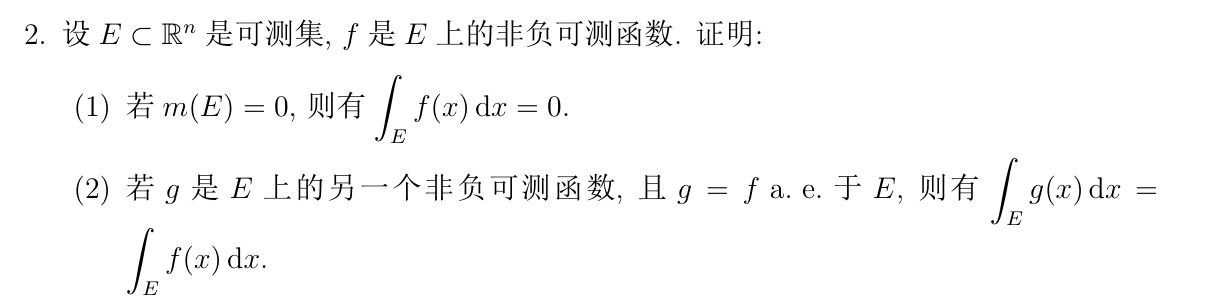
\includegraphics[width=\textwidth]{1-hw10-2025051210.png}
% \caption{}
\label{}
\end{figure}
\end{exercise}
\begin{proof}
(1)
$f\geq0$, denote $E_n=E(f\leq n)$, then
\[
\int_{E_n}^{} f(x) \, \mathrm{d}x \leq \int_{E_n}^{} n \, \mathrm{d}x =n\cdot m(E_n)\leq n\cdot m(E)=0\qquad \forall n\in \mathbb{N}
\]
Since $E=\bigcup_{n=1}^{\infty }E_n$,
\[
\begin{aligned}
\int_{E}^{} f(x) \, \mathrm{d}x  & =\int_{\mathbb{R}^{n}}^{} f(x)\chi_{E}(x) \, \mathrm{d}x  \\
 & \leq \int_{\mathbb{R}^{n}}^{} f(x)\sum_{n=1}^{\infty} \chi_{E_n}(x) \, \mathrm{d}x  \\
 & =\sum_{n=1}^{\infty} \int_{\mathbb{R}^{n}}^{} f(x)\chi_{E_n}(x) \, \mathrm{d}x  \\
 & =\sum_{n=1}^{\infty} \int_{E_n}^{} f(x) \, \mathrm{d}x  \\
 & =\sum_{n=1}^{\infty} 0 \\
 & =0
\end{aligned}
\]
(2)
\[
\begin{aligned}
\int_{E}^{} g(x) \, \mathrm{d}x  & =\int_{E(f=g)\cup E(f\neq g)}^{} g(x) \, \mathrm{d}x  \\
 & =\int_{E(f=g)}^{} g(x) \, \mathrm{d}x +\int_{E(f\neq g)}^{} g(x) \, \mathrm{d}x   \\
 & \overset{ m(E(f\neq g))=0 }{ = }\int_{E(f=g)}^{} g(x) \, \mathrm{d}x \\
 & =\int_{E(f=g)}^{} f(x) \, \mathrm{d}x \\
 & =\int_{E(f=g)}^{} f(x) \, \mathrm{d}x +\int_{E(f\neq g)}^{} f(x) \, \mathrm{d}x \\
 & =\int_{E(f=g)\cup E(f\neq g)}^{} f(x) \, \mathrm{d}x \\
 & =\int_{E }^{} f(x) \, \mathrm{d}x 
\end{aligned} 
\]
\end{proof}

\begin{exercise}
\begin{figure}[H]
\centering
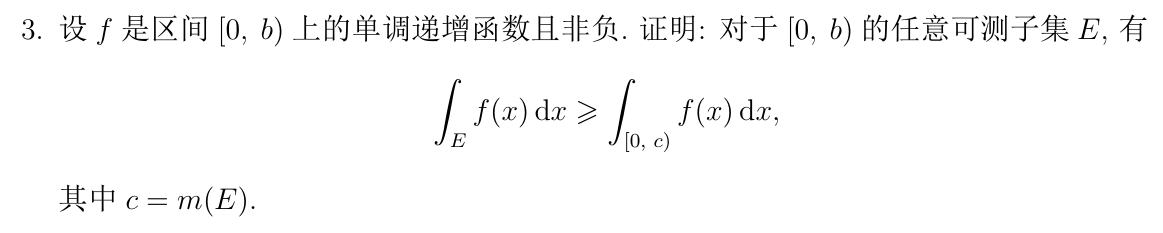
\includegraphics[width=\textwidth]{3-hw10-2025051210.png}
% \caption{}
\label{}
\end{figure}
\end{exercise}
\begin{proof}
Let $A\coloneqq E\setminus[0, c), B\coloneqq[0, c)\setminus E$, then
\[
m(E)=m(E\cap[0,c))+m(A)
\]
\[
m([0,c))=m(E\cap[0,c))+m(B)
\]
Since $m(E)=m([0,c))$, we have $m(A)=m(B)$; and
\[
\int_{E}f=\int_{[0,c)\cap E}f+\int_{A}f
\]
\[
\int_{[0,c)}f=\int_{[0,c)\cap E}f+\int_{B}f
\]
It suffices to show
\[
\int _{A}f\geq \int_{B}f
\]
For any $x\in A=E\setminus[0,c)=E\cap[c,b)$, $x\geq c$, as $f$ is monotonically increasing, $f(x)\geq f(c)$. Similarly, for any $x\in B$, $f (x)<f (c)$. Thus
\[
\int_{A}f\geq \int _{A}f(c)=f(c)\cdot m(A)\geq f(c)\cdot m(B)\geq \int_{B}f(c)\geq \int_{B}f
\]
We are done!
\end{proof}

\begin{exercise}
\begin{figure}[H]
\centering
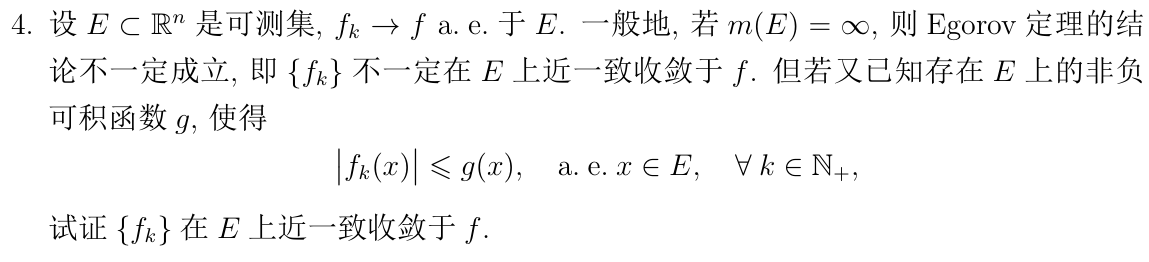
\includegraphics[width=\textwidth]{4-hw10-2025051210.png}
% \caption{}
\label{}
\end{figure}
\end{exercise}
\begin{note}
It's similar to the proof of Egorov theorem.
\end{note}
\begin{proof}
WLOG, assume that $f_n\to f$ on $E$, and $\lvert f_n \rvert\leq g$ on $E$, for any $k\in \mathbb{N}$; thus $\lvert f \rvert\leq g$ on $E$. Denote $h_n\coloneqq \lvert f_n-f \rvert$, then
\[
0\leq h_n=\lvert f_n-f \rvert \leq \lvert f_n \rvert +\lvert f \rvert \leq 2g
\]
$h_n$ is measurable, as $f_n,f$ are measurable. Construct sets
\[
A_{k,N}\coloneqq E\left( \sup_{j\geq N}h_j\geq \frac{1}{k} \right)=\bigcup_{j=N}^{\infty} \underbrace{ E\left( h_j\geq \frac{1}{k} \right) }_{ \in \mathcal{M} }\in \mathcal{M}
\]
Note that given $k$, we have $A_{k,N+1}\subseteq A_{k,N}$ for any $N$, thus $\{ A_{k,N} \}_{N=1}^{\infty}$ is \underline{descending} for each $k$; then
\[
\begin{aligned}
\bigcap_{N=1}^{\infty} A_{k,N} & =\lim_{ N \to \infty } A_{k,N} \\
 & =E\left( \lim_{ N \to \infty } \sup_{j\geq N}h_j\geq \frac{1}{k} \right) \\
 & =E\left( \varlimsup_{ j \to \infty } h_j\geq \frac{1}{k} \right) \\
 & \overset{ \lim_{ j \to \infty } h_j(x)=0,\forall x\in E }{ = }E\left( \lim_{ j \to \infty }h_j\geq \frac{1}{k}  \right) \\
 & =\varnothing
\end{aligned}
\]
Recall the continuity of measure for descending chain, we just need $m(A_{k,1})<\infty$ to show that\footnote{we haven't use  $g\in L^{1}(E)$ till now}
\[
\lim_{ N \to \infty } m(A_{k,N})=m\left( \bigcap_{N=1}^{\infty}A_{k,N}  \right)=m(\varnothing)=0
\]
\begin{note}
If $m(E)<\infty$, then $m(A_{k,1})\leq m(E)<\infty$, which is Egorov theorem; if $m(E)=\infty$, but $h_j$ is controlled by $2g\in L^{1}(E)$, we can also prove $m(A_{k,1})<\infty$.
\end{note}
\[
\begin{aligned}
m(A_{k,1}) & =m\left( E\left( \sup_{j\geq 1}h_j\geq \frac{1}{k} \right) \right) \\
 & =k\cdot\frac{1}{k}\cdot \int_{E\left( \sup_{j\geq 1}h_j\geq \frac{1}{k} \right)}^{} 1 \, \mathrm{d}x  \\
 & \leq k \int_{E\left( \sup_{j\geq 1}h_j\geq \frac{1}{k} \right)}^{} \sup_{j\geq 1}h_j \, \mathrm{d}x  \\
 & \leq k\int_{E\left( \sup_{j\geq 1}h_j\geq \frac{1}{k} \right)}^{} 2g \, \mathrm{d}x \\
 & \leq 2k\underbrace{ \int_{E}^{} g(x) \, \mathrm{d}x }_{ <\infty } <\infty
\end{aligned}
\]
The following steps are routine.

For any $\delta>0$, there exists $N_k>0$ for each $k$, s.t.
\[
m(A_{k,N_k})<\frac{\delta}{2^{k}}
\]
Let $F\coloneqq\bigcup_{k=1}^{\infty}A_{k,N_k}$, then
\[
m(F)=m\left( \bigcup_{k=1}^{\infty} A_{k,N_k} \right)\leq \sum_{k=1}^{\infty} m(A_{k,N_k})\leq \sum_{k=1}^{\infty} \frac{\delta}{2^{k}}=\delta
\]
Let $E_{\delta}=E\setminus F$, then $m(E\setminus E_{\delta})=m(F)\leq\delta$, we verify that $f_n\rightrightarrows f$ on $E_{\delta}$.

For any given $\epsilon>0$, pick $k_0\in \mathbb{N}$ s.t. $\frac{1}{k_0}<\epsilon$. For any $x\in E_{\delta}=E\setminus F$, $x\not\in A_{k,N_k}$ for any $k$; thus $x\not\in A_{k_0,N_{k_0}}$; $\sup_{j\geq N_{k_0}}h_j(x)<\frac{1}{k_0}<\epsilon$, i.e.
\[
\lim_{ N \to \infty } \sup_{x\in E_{\delta}}\lvert f_{N}(x)-f(x) \rvert =0 
\]
i.e. $f_n\rightrightarrows f$ on $E_{\delta}$. We are done!
\end{proof}

\begin{exercise}
\begin{figure}[H]
\centering
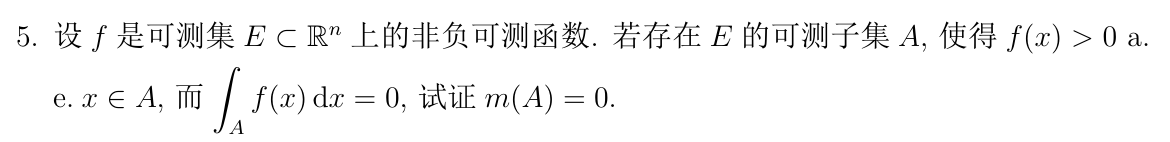
\includegraphics[width=\textwidth]{5-hw10-2025051210.png}
% \caption{}
\label{}
\end{figure}\label{34ffe7}
\end{exercise}

\begin{proof}
\[
m(A(f=0))=0
\]
\[
A=A(f>0)\cup A(f=0)
\]
\[
\begin{aligned}
\int_{A}^{} f(x) \, \mathrm{d}x  & =\int_{A(f>0)\cup A(f=0)}^{} f(x) \, \mathrm{d}x  \\
 & =\int_{A(f>0)}^{} f(x) \, \mathrm{d}x +\int_{A(f=0)}^{} f(x) \, \mathrm{d}x  \\
 & =\int_{A(f>0)}^{} f(x) \, \mathrm{d}x \\
 & \geq \int_{A(f>0)}^{}  1\, \mathrm{d}x  \\
 & =\int_{A(f>0)}^{}  1\, \mathrm{d}x+\underbrace{ \int_{A(f=0)}^{} 1 \, \mathrm{d}x   }_{ =m(A(f=0))=0 } \\
 & =\int_{A}^{} 1 \, \mathrm{d}x  \\
 & =m(A)
\end{aligned}
\]
Then
\[
m(A)\leq \int_{A}^{} f(x) \, \mathrm{d}x =0\implies m(A)=0
\]
\end{proof}

\begin{exercise}
\begin{figure}[H]
\centering
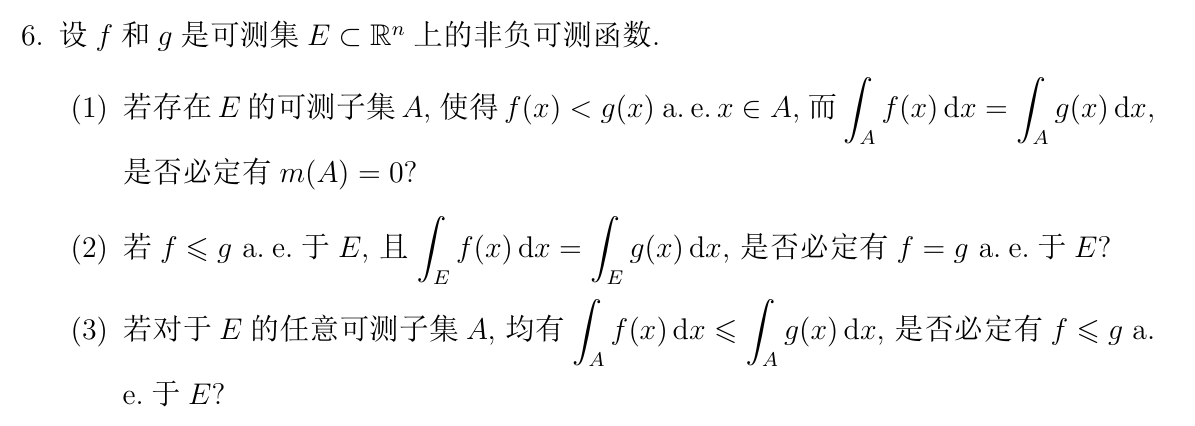
\includegraphics[width=\textwidth]{6-hw10-2025051210.png}
% \caption{}
\label{}
\end{figure}
\begin{figure}[H]
\centering
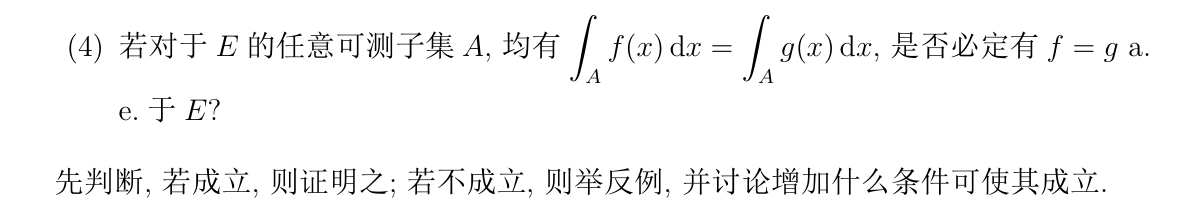
\includegraphics[width=\textwidth]{7-hw10-2025051210.png}
% \caption{}
\label{}
\end{figure}
\end{exercise}
\begin{proof}
(1) false, consider $E=A=\mathbb{R}^{n}$, $f\equiv1$, $g\equiv2$. This is true when
\[
\int_{A}^{} f(x) \, \mathrm{d}x =\int_{A}^{} g(x) \, \mathrm{d}x <\infty
\]
(2) fasle, consider $E=A=\mathbb{R}^{n}$, $f\equiv1$, $g\equiv2$. This is true when
\[
\int_{E}^{} f(x) \, \mathrm{d}x =\int_{E}^{} g(x) \, \mathrm{d}x <\infty
\]
(3) true, if $m(E(f>g))>0$, then
\[
\int_{E(f>g)}^{} f \, \mathrm{d}x >\int_{E(f>g)}^{} g \, \mathrm{d}x 
\]
(4) true, from (3) we know that $f\geq g$ a.e. and $f\leq g$ a.e. thus $f=g$ a.e.
\end{proof}

\begin{exercise}
\begin{figure}[H]
\centering
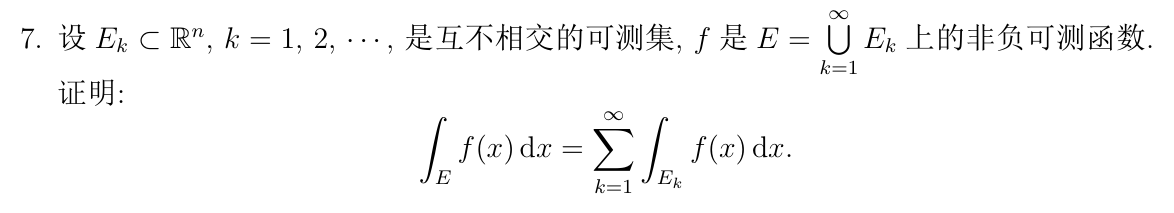
\includegraphics[width=\textwidth]{8-hw10-2025051210.png}
% \caption{}
\label{}
\end{figure}
\end{exercise}
\begin{proof}
\[
f_n\coloneqq f\cdot \chi_{\bigcup_{k=1}^{n} E_k}
\]
Then
\[
f_1\leq f_2\leq \dots\leq f_n\leq f_{n+1}\leq \dots
\]
By Beppo Levi's theorem,
\[
\lim_{ n \to \infty } \int_{E}^{} f_n(x) \, \mathrm{d}x=\int_{E}^{} \lim_{ n \to \infty } f_n(x) \, \mathrm{d}x
\]
i.e.
\[
\lim_{ n \to \infty } \int_{E}^{} f\cdot \chi_{\bigcup_{k=1}^{n} E_k} \, \mathrm{d}x =\int_{E}^{} f\cdot \chi_{\bigcup_{k=1}^{\infty} E_k} \, \mathrm{d}x =\int_{E}^{} f \, \mathrm{d}x 
\]
\[
\lim_{ n \to \infty } \int_{E}^{} f\cdot \chi_{\bigcup_{k=1}^{n} E_k} \, \mathrm{d}x =\lim_{ n \to \infty } \int_{\bigcup_{k=1}^{n} E_k}^{} f \, \mathrm{d}x =\lim_{ n \to \infty } \sum_{k=1}^{n} \int_{E_k}^{} f \, \mathrm{d}x =\sum_{k=1}^{\infty} \int_{E_k}^{} f \, \mathrm{d}x
\]
Therefore,
\[
\sum_{k=1}^{\infty} \int_{E_k}^{} f \, \mathrm{d}x =\int_{E}^{} f \, \mathrm{d}x
\]
\end{proof}

\begin{exercise}
\begin{figure}[H]
\centering
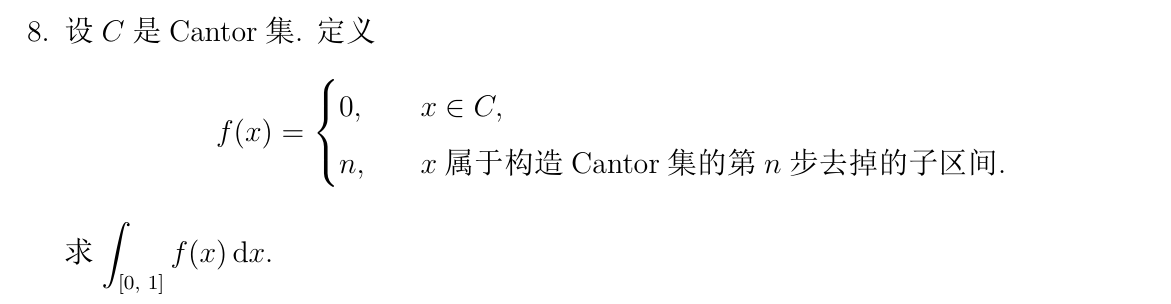
\includegraphics[width=\textwidth]{9-hw10-2025051210.png}
% \caption{}
\label{}
\end{figure}
\end{exercise}
\begin{proof}
\[
\int_{[0,1]}^{} f(x) \, \mathrm{d}x =\sum_{n=1}^{\infty} \frac{n \cdot2^{n-1}}{3^{n}}=3
\]
\end{proof}
